%!TEX root = ../../thesis.tex
\section{Scheduling}
\label{sec:impl-scheduling}

The scheduling system is a major backbone of any audio editing software. The playback of buffers and the timing of drum machines and synthesizers needs to be exact to the millisecond. Timing glitches cause unwanted effects on arrangements and can destroy the playback experience of a song. Inexact timing will also frustrate users because it is an error that renders the usage of the editor for song composition impossible.

As already described in \refchapter{subsec:timing-in-web-audio}, the Web Audio API provides an exact timing system. This system, however, does not provide a scheduler, it only comes with a way to exactly time individual Web Audio components and nodes (e.g. buffers and oscillators). All custom components (e.g. drum machines) need a custom timing component that builds on top of the provided timing methods. Not only do all custom components need their own timing mechanism but also the overall arrangement, which contains information on when to play which piece of a track.

A na\"ive approach to implement a scheduler for an arrangement would be to calculate the start time for all pieces and to start them all when the user initiates the playback. All individual nodes would then play at the precisely calculated time and the arrangement playback would be perfect. Nonetheless, this approach comes with some drawbacks.

Firstly, the scheduler would need to hold references to each node and its subnodes in memory in order to stop them when the user stops the playback of the arrangement. This also implies that all nodes would need to be created initially, which could, for a complex arrangement, take a non-trivial amount of time. Both issues also lead to a constant high usage of memory that might affect the performance of the editor.

Secondly, although it is not stated in the Web Audio specification\footnote{\cite{wilson2014webaudiospec}}, the initial very high amount of pre-scheduled audio events could have a negative impact on the audio playback and also the editor's performance. Scheduling each node upfront means that each individual sound of a drum machine would need to be scheduled upfront as well. This could, depending on the arrangement and used audio nodes, result in thousands of pre-scheduled nodes.

In order to have playback control over all these nodes, they would need to be kept in memory. The iteration over each individual node can take a non-trivial amount of CPU time which would block the main user interface thread. The editor's user interface needs to stay responsive and interactive the whole time. A negative scenario would be that the user interface would not react and freeze when the user wants to seek to a different position in the arrangement by clicking the position in the timeline element. All scheduled audio events would need to be stopped and restarted when seeking to a different point in the arrangement.

\subsection{Arrangement Scheduler}

For all the above mentioned reasons, a more complex scheduling system is needed that ensures that the following requirements are fulfilled:

\begin{enumerate}
  \item All sounds need to be timed precisely.
  \item The system needs to have a small memory footprint.
  \item The system does not block the main user interface.
\end{enumerate}

The main problem of the na\"ive scheduler was that it had to schedule and allocate all events at once, which led to many problems. Most of these problems can be overcome by introducing a gradual scheduler which schedules sounds depending on the current position in the playback of the arrangement. The basis for this scheduler is a combination of JavaScript's own timing methods (compare \refchapter{subsec:timing-in-js}) and the precise timing methods in the Web Audio API.

\begin{figure}[htb]
  \centerline{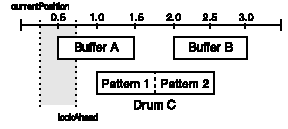
\includegraphics[width=0.9\linewidth]{images/Scheduler_Example.pdf}}
  \caption[Scheduler]{Scheduler}
  \label{fig:scheduler}
\end{figure}

\reffigure{fig:scheduler} shows an example arrangement with a Buffer that should be played at 0:00,5 minutes (Buffer A), another Buffer that should be played at 0:02 minutes and a drum machine, containing 2 patterns, which should start at 0:01 minutes.

The scheduler uses a \code{Ticker} object to gradually check if new pieces need to be scheduled. A \code{Ticker} uses JavaScript's \code{setInterval} to constantly notify listeners that a new interval has passed. So whenever an interval has passed, the scheduler scans the arrangement for unscheduled pieces using the following algorithm (\reflisting{lst:scheduling-pieces-p1}):

\begin{lstlisting}[language=JavaScript, caption=Detecting pieces that need to be scheduled, label=lst:scheduling-pieces-p1]
  for(piece in unscheduledPieces){
    var inLookahead = position < piece.position &&
                      position + lookAhead >= piece.position;

    var inBetween = position >= piece.position &&
                    position < piece.position + piece.length;
    (...)
  }
\end{lstlisting}

First, the scheduler checks if the current piece starts in the \code{lookAhead} window (line 2f). Therefore, the current \code{position} in the song, which is as well calculated in each interval, is compared to the piece's starting \code{position} and the \code{lookAhead} time frame. If the song \code{position} plus the \code{lookAhead} time is more or equal than the piece's \code{position}, the piece needs to be scheduled in this time frame. By using a \code{lookAhead} time comparison, the scheduler ensures that even in the case of a large delay in the \code{Ticker's} \code{setInterval}, all pieces will be scheduled correctly and none of them is skipped. Consequently, the \code{lookAhead} time is a multiple of the \code{Ticker's} interval time. The current implementation uses a \code{lookAhead} of three times the interval. The interval time itself is set to the shortest length of all pieces to ensure that no piece can be skipped by a interval that is too long and also to reduce the overall amount of timeouts, e.g. if a too short interval is chosen. In case of a song position of 0:01 minutes, only Buffer A would be scheduled initially.

This first check alone already ensures that the number of simultaneously scheduled pieces is reduced to the bare minimum. But it does not cover several edge cases and would also schedule all pieces that start before the current song position, even if the scheduler was started with a song position after their position in the song such as when the scheduler was started at 0:01,6 seconds and Buffer A would be scheduled as well, although it does not need to be scheduled.

The second check (line 5f) ensures to leave out pieces that ended before the scheduler was started by comparing the song \code{position} to the \code{piece's position} plus its \code{length}, which is the end time of the current piece. When the song's \code{position} is less than the end time of the piece and the song \code{position} is bigger than or equal to the \code{piece's position}, the scheduler sorts out ended pieces. In addition to that, the scheduler selects pieces that need to be scheduled with an offset. This case happens when the scheduler is started at a song position that lays between the beginning and the end of a piece, e.g. if the scheduler in \reffigure{fig:scheduler} would start with a song position of 0:01 minutes. Buffer A would need to be scheduled with an offset.

\begin{lstlisting}[language=JavaScript, caption=Scheduling pieces, label=lst:scheduling-pieces-p2]
  if(inLookahead || inBetween){
    var when = Math.max(piece.position - position, 0);

    var offset = Math.max(position - piece.position, 0);

    piece.start(when, offset);
    scheduledPieces.push(piece);
  }
\end{lstlisting}

If either the first or the second check was truthy, the piece will be scheduled (line 1, \reflisting{lst:scheduling-pieces-p2}). The exact point \code{when} to start the piece is calculated from the difference of the \code{song's position} and the \code{piece's position} (line 2). Also, in case the piece needs to be started with an offset, the offset is calculated by subtracting the \code{piece's position} from the current song \code{position} (line 4). In the last step, the piece is started and added to the list of scheduled pieces. The list of scheduled pieces is needed for the case that the user stops the playback of the arrangement and all scheduled pieces need to be stopped so that they do not play.

The described scheduling system does fulfill all three requirements. By using the \code{lookAhead} method it ensures that even if the system uses the inaccurate \code{setInterval} function, all pieces are scheduled precisely and also calculates offset positions. The overall memory footprint is very small because the system only keeps already scheduled top-level pieces (see \refchapter{subsec:local-scheduler}). Lastly, the system does not block the main user interface thread because cancelling pieces is very fast (due to the low amount of pieces) and the scheduling mechanism is triggered intelligently only when really needed.

\subsection{Local Scheduler}
\label{subsec:local-scheduler}

The intelligently selected interval of the above described scheduler solely reduces the computation time if only top-level pieces are handled. This works well for recorded pieces, but not so well for drum machine pieces or synthesizer pieces because the minimum interval time for these pieces would actually be much lower. These pieces are composed of many individual sounds with only a friction of a second delay in between them, which would lead to a lot more scheduling intervals and therefore to a much higher CPU usage. For this reason, these pieces have their own schedule-mechanism, which is triggered by the above shown arrangement scheduler. The arrangement scheduler is not aware of the fact that, for example, drum machine pieces are different from recorded pieces, because they share the same interface and can be triggered in the same way. They both have a \code{start} method (compare \reflisting{lst:scheduling-pieces-p2}, line 6) that accepts a point in time (\code{when}) and an \code{offset}. So the complexitiy behind the ``local scheduler'' is not exposed to the ``global scheduler'' (the arrangement scheduler).

\begin{figure}[htb]
  \centerline{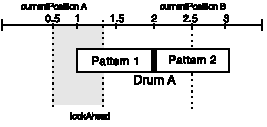
\includegraphics[width=0.9\linewidth]{images/Scheduler_Example_Drum.pdf}}
  \caption[Scheduler and sampler]{Scheduler and sampler}
  \label{fig:scheduler-sampler}
\end{figure}

All pieces that need an own scheduling mechanism are organised into patterns (see \refchapter{impl-drum-machine}), which themselves consist of the individual sounds and their timing information. These pieces use a sampler for their internal scheduling. \reffigure{fig:scheduler-sampler} shows an example of an arrangment with a drum machine (Drum A) that is composed of two patterns (Pattern 1 and Pattern 2). The global scheduler starts at 0:00,5 minutes and sees that Drum A needs to be scheduled to start in 0.5 seconds and calls the drum machine's \code{start} method. Behind the scenes it is not the drum machine's method but the drum machine's sampler's \code{start} method. The sampler also, just as the global scheduler, uses a \code{Ticker} object to gradually schedule notes or, more precisely, to gradually schedule patterns. One of the requirements for the scheduler is to have as few interval timeouts as possible to reduce the CPU usage. If the sampler were to schedule individual notes, the minimal interval time would be very low and would result in a lot of timeouts and extra calculation. Also, the offset error rate for small timeouts has a much bigger impact on the complexity of achieving an accurately timed playback than for bigger timeouts. For this reason, the sampler schedules whole patterns at once.

\begin{lstlisting}[language=JavaScript, caption=Scheduling patterns (sampler), label=lst:scheduling-patterns]
  if(this.hasNextPattern()){
    if((currentTime + lookAhead) > this.nextPatternTime()){
      this.scheduleNextPattern();
    }
  }else{
    cleanUpMemory();
  }
\end{lstlisting}

Similar to the global scheduler, the sampler uses a \code{lookAhead} time in order to determine if a pattern needs to be scheduled (line 2, \reflisting{lst:scheduling-patterns}). If a next pattern is detected and needs to be scheduled, all notes of that pattern are scheduled ahead (line 3). Otherwise, if there is no next pattern, the sampler can clean up the memory (line 6). This needs to be done, because references to all scheduled notes are kept in memory for the currently playing pattern to be able to stop them, when playback is stopped. Othwerwise, all scheduled drum notes would play even if the user has pressed the stop button. The calculation of the startup time for each note depends either on the drum machine's BPM or the position of the note in a synthesizer's arrangement.

In addition to pattern scheduling, the sampler also takes care of calculating the impact of offsets for each pattern. In \reffigure{fig:scheduler-sampler}, \code{currentPosition B} shows an example where a sampler needs to take an offset into its scheduling calculation. In this case, Drum A will be scheduled with an offset of 1.5 seconds which means that the sampler needs to schedule Pattern 2 and not Pattern 1. The sampler also needs to leave out all notes that were played before \code{currentPosition B}.

\begin{lstlisting}[language=JavaScript, caption=Calculating offsets (sampler), label=lst:scheduling-offsets]
  function(offset){
    forEachPatternInOrder(function(pattern, index){
      patternEnd += pattern.length;

      if(offset < patternEnd + pattern.length){
        currentPattern = pattern;
        return false;
      }else{
        patternEnd += pattern.length;
      }
    });

    var patternOffset = offset -
                (patternEnd - currentPattern.length);
    var beat = patternOffset /
                currentPattern.secondsBetweenBeats();

    beat = Math.floor(beat);
    currentPattern.beat = beat;
  }
\end{lstlisting}

The algorithm in \reflisting{lst:scheduling-offsets} is initialized with the \code{offset} that was determined from the global scheduler (line 1). As a first step, the algorithm detects the correct pattern from the pattern order that should be played at the current offset position (line 2ff). The current pattern lengths are summed up until the offset has been reached (line 5). After that, the relative offset of the current pattern is determined by subtracting the length until the current pattern (line 14) from the global \code{offset} has been reached, which results in the time that should be skipped for the current pattern. In case of the example in \reffigure{fig:scheduler-sampler} (\code{currentPosition 2}), the \code{patternOffset} should be 0.5 seconds. The step after that is different for the drum machine's sampler and the synthesizer's sampler but for reasons of simplicity, \reflisting{lst:scheduling-offsets} only shows the former implementation for note skipping. Through dividing the \code{patternOffset} by the current pattern's BPM (converted to seconds per beat), the algorithm is able to detect the amount of beats that need to be skipped (line 15f). This beat is then used as the base beat for the current pattern (line 19) and all beats before that will be skipped. The synthesizer's sampler uses a combination of all the above described techniques to determine the skipped notes and explaining it here would only repeat already covered implementation details.

The local scheduler ensures that all three requirements for an efficient scheduler are met. It adds a precises timing method for drum machines and synthesizers by pre-scheduling complete patterns. Although all played notes are held in memory for a short time, the \code{cleanUpMemory} method assures that unused notes are released to keep the memory footprint small. Lastly, the scheduling interval timeouts are kept to a minimum in order to reduce CPU usage.
